\chapter{Background}\label{ch:Background}

% This chapter provides some background research on the project and examines some previous work.
% what does the reader need to understand this work
This Chapter introduces a body of knowledge from domains intersecting the overarching aim of this work, providing the reader with the necessary tools to dissect the components presented throughout the thesis. This Chapter begins from introducing basic sound physics, wave theory, and human perception as they define basic concepts of auditory interactions in the physical and in virtual worlds.\par
Since a human listener is a link in the chain of the system proposed as part of this work, this Chapter will introduce some 

\section{Background on Human Hearing}
\subsection{Characteristics of the Human Hearing System}
The \acrfull{has} generally comprises two ears on either side of the human head, and each ear is a system that can be divided into three main parts: the outer ear, commonly referred to as the ear; the middle ear; and the inner ear. The outer ear, also referred to as the pinna, is shaped like a shell, is made of cartilage and skin, and serves both as protection for the system of receptors, ossicles, and nerves within the middle and the inner ear and a funnel that collects sound energy and transmits it to the middle ear via the outer ear canal. The outer ear canals are largely responsible for the frequency response of the \acrshort{has}. 
Auditory stimuli are sent to the brain via sensory cells that are surrounded by fluids displacing according to the received sound pressure. The middle ear converts sound pressure from the ear canal to displacement to these fluids, which send signals to the brain. This part of the ear is able to withstand variations of air pressure arriving at the outer ear and is responsible for matching different impedance magnitudes between the air or the medium in which sound is arriving at the apparatus and the impedance of the fluids in the inner ear.
The inner ear comprehends the vestibular system, a sensory system that allows humans to sense their spatial position, perceive rotation or displacement, and achieve balance and the cochlea. The cochlea, shaped like a snail, is embedded in the hard temporal bone, part of the skull.
\begin{figure}
    \centering
    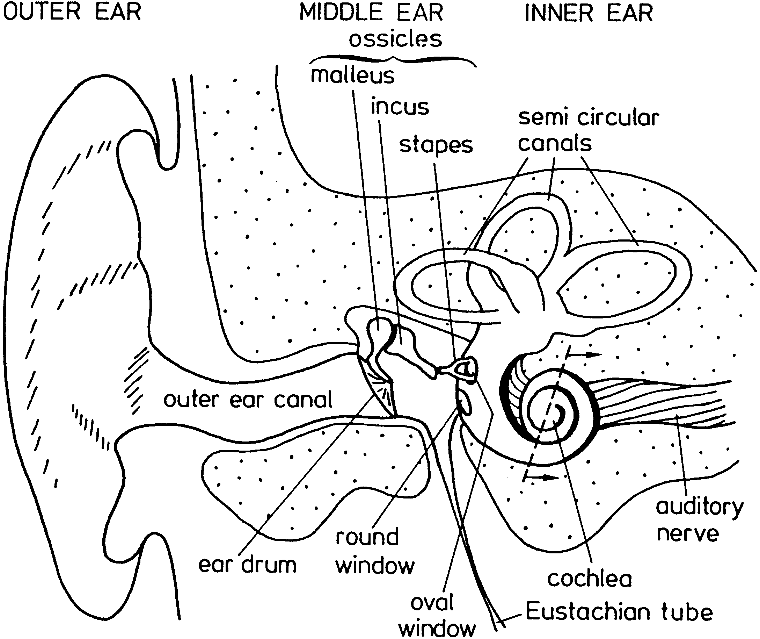
\includegraphics[width=1\linewidth, trim={0cm 0cm 0cm 0cm}, clip]{human_ear}
    \caption[Overview of the human hearing system]{Overview of the human hearing system \citep{zwicker2013psychoacoustics}}
    \label{fig:human_hearing_system}
\end{figure}

\cite{zwicker2013psychoacoustics}


\subsection{Introduction to Psychoacoustics}\label{sec:bg-psychoacoustics}
The \acrshort{has} enables one of the fundamental functions of perception of surrounding space. In humans and species of the animal kingdom, hearing is the basis of many mechanisms, such as communication or survival instincts. Such mechanisms are neural processing applied to auditory stimuli arriving at the hearing system in order to compute tasks or solve problems, such as communicating using acoustical data or pinpointing the location of a sound-emitting entity relying on auditory stimuli. These are example applications or problems that can be solved by processing acoustical data interpreted by the \acrshort{has}.
Psychoacoustics investigates how the \acrshort{has} responds to auditory stimuli and investigates applications like loudness perception, localisation, lateralisation, or room volume estimation. The understanding of psychophysical responses of the \acrshort{has} to acoustical data in environments influences everyday activities that involve communicating, listening to musical instruments, or delivering messages to an audience of multiple listeners. The design process of built environments, infrastructure, or concert halls takes into account psychoacoustic factors to facilitate or improve human perception in specific environments during specific activities.

\subsection{Sound Localisation}
\begin{figure}
    \centering
    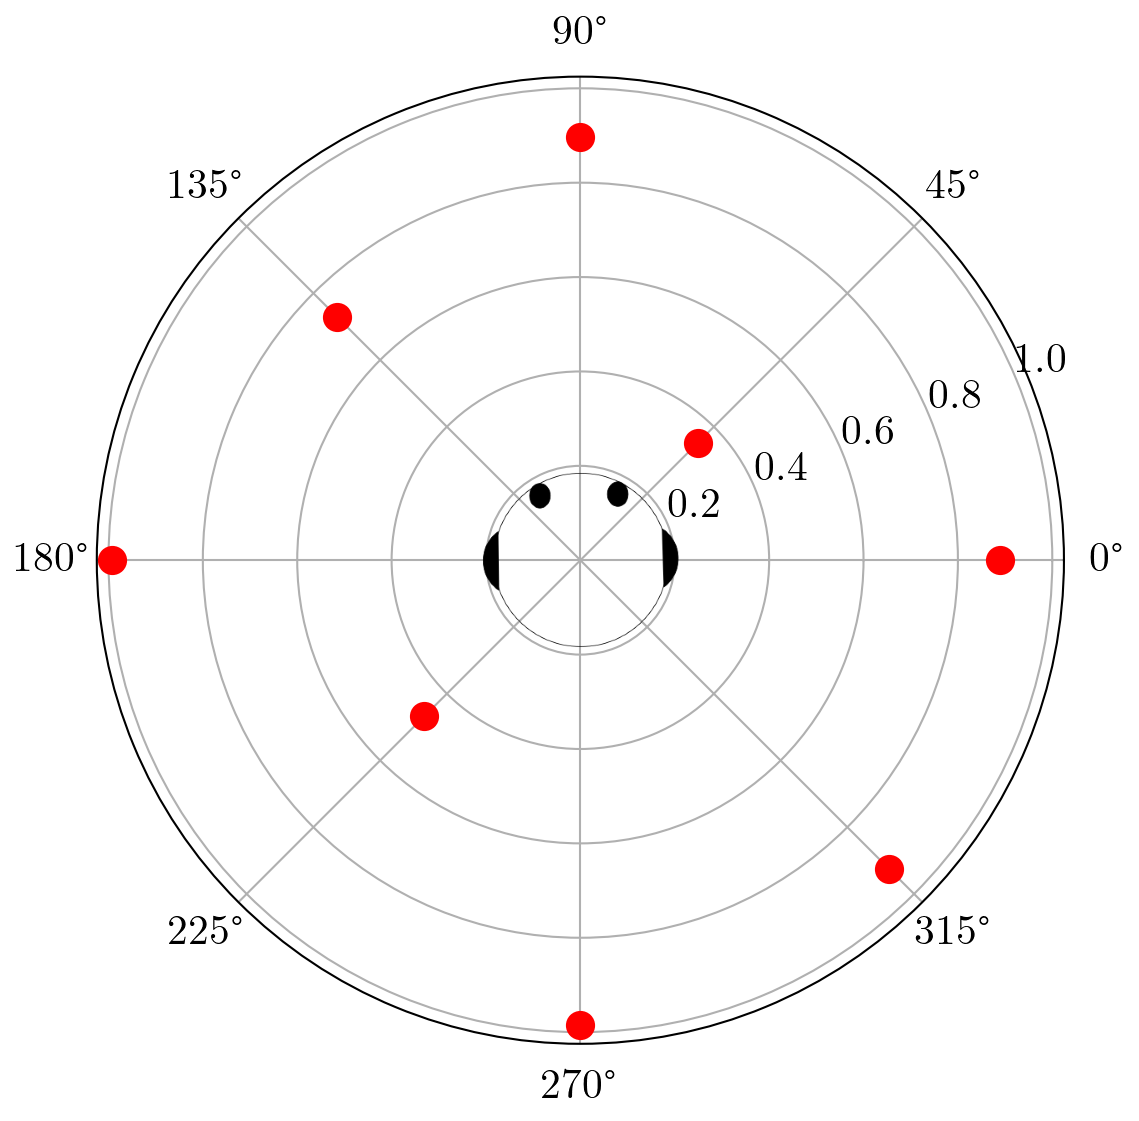
\includegraphics[width=1\linewidth]{localisation_example}
    \caption{Sound localisation is the ability of the \acrshort{has} to pinpoint the position and direction of sound sources, red dots, at different directions and distances around the listener, centre.}
    \label{fig:localisation-listener}
\end{figure}

\section{Acoustic Theory}
\subsection{Wave theory}
Sound propagation is a transmission of energy in a sound field, which can be thought of as a superposition of sound waves travelling in a medium. In this work, we consider air as the sound propagation medium, which is assumed to be homogeneous, i.e., determining a constant velocity of sound $c$ expressed as: 
\begin{equation}
c = (331.4 + 0.6\Theta)~\frac{m}{s}   
\end{equation}
where $\Theta$ is the temperature in centigrade.
A vibrating object in a sound field causes air particles to move, initiating the transmission of energy in the field. Such an object is defined as a sound source, and if the intensity and frequency of the vibrations are within the perceptible range of the human hearing system, a listener may experience sound emitted by the said sound source.
In everyday sound transmissions, the air within sound fields is not at rest and features many inhomogeneities caused by external factors affecting the state of its particles, such as windows or air conditioning systems. However, according to \citep{kuttruff2016room}, such inhomogeneities are imperceptible, and generally, the air temperature has a perceptual effect on sound transmissions, especially in large concert halls and open spaces. Air temperature effects can be neglected in indoor sound propagation.

\subsection{Sound Transmissions}
Energy in the sound field, transferring from a vibrating sound source to the hearing system of a listener, is perceived as an acoustic signal characterised by varying intensity and frequency. 
The intensity of 
Sound pressure, amplitude, sampling 

\subsection{Acoustics in Real Environments}
\begin{itemize}
    \item Definition of a sound field
    \item Characterisation of sound fields
    \item Objective metrics describing sound fields; Farina's descriptors.
    
\end{itemize}


\section{Digital Representation of Audiovisual Information}
\label{sec:DSP-background}
The following section will introduce background knowledge on Digital Signal Processing relevant to the representation of acoustic signals in digital systems and the manipulation of auditory stimuli in virtual environments. Digital Signal Processing methods and techniques provide building blocks for the construction of realistic 3D auditory displays in immersive technology.

\subsection{Digital Signal Processing for Acoustic Rendering}
Digital Signal Processing (DSP) is the science of analysing time-dependent physical processes. The acoustics realm deals with analogue signals and digital signals, terms used to indicate a continuous variation of amplitude values in a physical process. Electricity utilised to drive loudspeakers is an example of an analogue signal, expressing continuous changes in voltage applied to magnets to displace the position of a cone. The cone displacement causes pressure differences in air particles, transforming such changes in voltage to changes in air pressure, which the human auditory system interprets as sound. Acoustic signals consist of one or multiple sound waves oscillating, where each wave is an oscillation of energy at regular intervals; the duration of each interval determines the wavelength $\lambda$, and oscillations are measured as frequency in Hertz (Hz). \par
On the other hand, a digital signal is a discrete representation of a continuous physical process, resulting in a sequence of measurement samples of an analogue signal expressed as amplitude values over time. Figure 1 shows the difference between a continuous signal and a discrete signal: digital signal is represented with stems to indicate its nature of quantised measurements over time, abscissa, as opposed to a continuous change in amplitude, ordinate. The discrete nature of a digital signal has inherent problems and advantages that relate to the time interval between measurements: a digital signal representing an analogue one will always be an approximation of the continuous process as the system may change its state between measurement intervals. The approximated nature of digital signals causes information loss, which is counteracted by theories shown later, but allows digital systems to store and process acoustical data efficiently.\par
DSP applies to both, but in this book chapter, we will only focus on the branch of DSP that deals with digital signals. Digital systems like computers are used to process stored acoustical signals for several reasons, such as storing recordings of anechoic acoustic signals that simulation software can then process to generate realistic acoustic simulations, expressed as a processed digital signal. \par
\begin{figure}
    \centering
    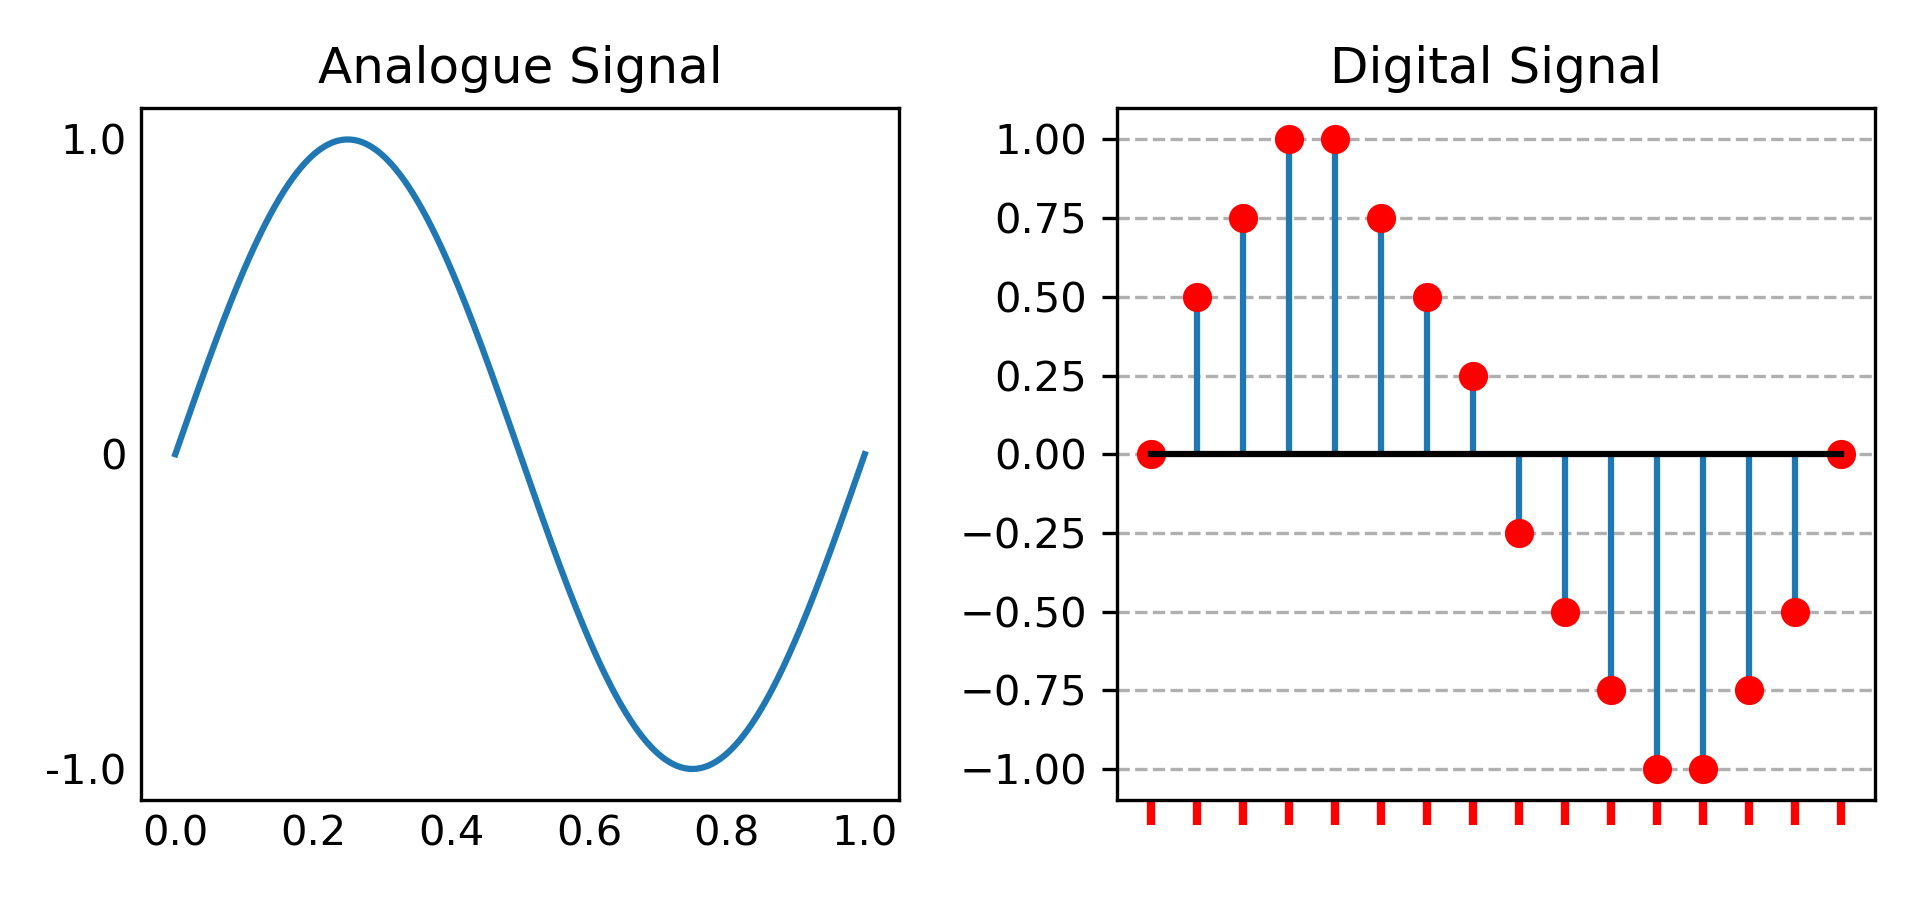
\includegraphics[width=1\linewidth]{analogue_digital}
    \caption{Analogue and digital signal: the left axes show a continuous signal, and the right axes show a discrete sampled representation.}
    \label{fig:analogue-digital-signal}
\end{figure}

The process of converting continuous signals to digital information involves taking measurements of the amplitude of a continuous signal at regular time intervals. There are two dimensions in which the analogue signal is measured during this process, the amplitude and time, respectively, the abscissa and the ordinate of Figure~\ref{fig:analogue-digital-signal}.\par
Due to the physical limitations of digital technology, A/D converters can only take a finite number of measurements between time intervals, and they have limited accuracy in representing amplitude levels. In Figure \ref{fig:analogue-digital-signal}-b, it is possible to see how an A/D converter sees analogue signals: given an acoustic continuous signal as input, it takes amplitude samples at every time step, marked with by red ticks, and measures using the available amplitude levels (the dotted horizontal lines). As a result, the process outputs a series of data points, the red dots, approximating the input, and the resolution and fidelity of the approximation depend on the time elapsed between time steps and the available amplitude level points. There are standards to ensure the reproduction and manipulation of acoustical signals in digital systems with an appropriate fidelity, such as the ``Red Book'' IEC 60908 standard, adopted for the Compact Disc music format, determining that digital signals must be represented by 44.100 measurement samples per second, at 16bit amplitude resolution. 16-bit refers to the binary representation adopted by digital systems to store amplitude values, allowing $2\textsuperscript{16}=65,535$ possible amplitude levels. The sampling frequency, the number of measurements per second, is calculated in Hertz (Hz), and it is a fundamental property of digital signals that must be taken into account for almost all types of audio manipulation and analysis involved in acoustical applications and it paramount to correct reconstructions of any acoustic information in any digital system. \par
The Nyquist-Shannon sampling theorem is used to ensure a digital system reconstructs an analogue signal correctly. The theorem proves that a wave must be sampled at least twice during each oscillation period. A periodic wave oscillating at $20kHz$, which is around the maximum perceivable frequency in the human hearing range, would need to be sampled at least $40,000$ per second; hence, the standard $44.1kHz$ sampling rate. In Figure~\ref{fig:aliasing}, for instance, a $50Hz$ signal is sampled at $90Hz$, below the $100Hz$ Nyquist sampling frequency, causing aliasing, an incorrectly reconstructed signal that will be able to oscillate at a maximum frequency of $45Hz$.\par

\begin{figure}
    \centering
    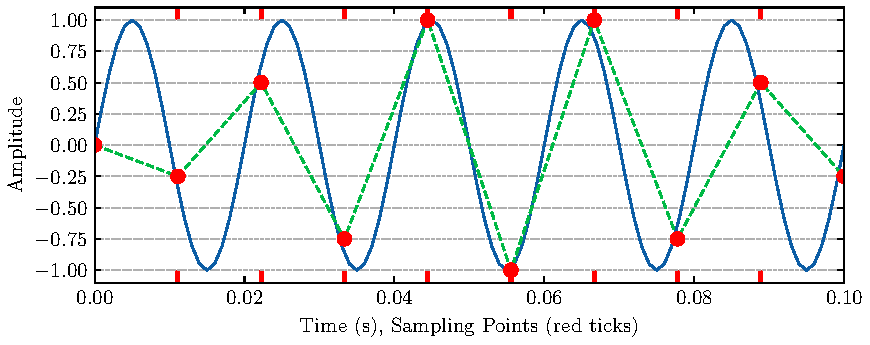
\includegraphics[width=1\linewidth]{aliasing}
    \caption{The blue signal is being sampled at a sampling frequency lower than the Nyquist frequency, causing aliasing, an incorrect reconstruction of the digital signal, as opposed to Figure~\ref{fig:analogue-digital-signal} that shows a correctly reconstructed signal. As a result, the dotted green signal is created instead, having a frequency between $0Hz$ and the sampling frequency.}
\label{fig:aliasing}
\end{figure}

\subsubsection{Analysis of Digital Signals}
Acoustical signals are often analysed in the time domain, as varying sound pressure levels over time, or in the frequency domain. By considering acoustical signals as a Fourier series, a function composed of sine or cosine primitives, the frequency domain representation determines how the power of an acoustical signal is distributed in a range of sine and cosine functions with wavelengths usually ranging from the minimum to the maximum perceivable frequencies of the human auditory system - low to high frequencies. Time- and frequency-domain representations are often used for both analysis and manipulation of acoustical signals, often adopted in tasks like determining the effects of an environment in the perception of sound emitted by an object and arriving to a listener in said environment \cite{ballou2013handbook}. \par 
In acoustics for interactive applications, engineers often adopt the Discrete-Time Fourier Transform (DTFT), a Fourier series for digital signals, which is one of the fundamental concepts in DSP. It takes a sequence, such as the signal represented in Figure\ref{fig:analogue-digital-signal}-b and generates $N$ complex numbers, representing power across $N$ sinusoids. The DTFT, as defined by classic DSP theory \cite{shenoi2005introduction}, transforms a signal $x_n$ containing samples $x_0, x_1,~\dots, x_{N-1}$ into a series $X_k$ of complex numbers $X_0, X_1,~\dots, X_{N-1}$. $X_k$ is defined by:
\begin{equation}
    X_k = \sum_{n=0}^{N-1} x_n~\cdot~e^{-\frac{i2\pi}{N}kn}
\end{equation}

\begin{figure}[htb]
    \centering
    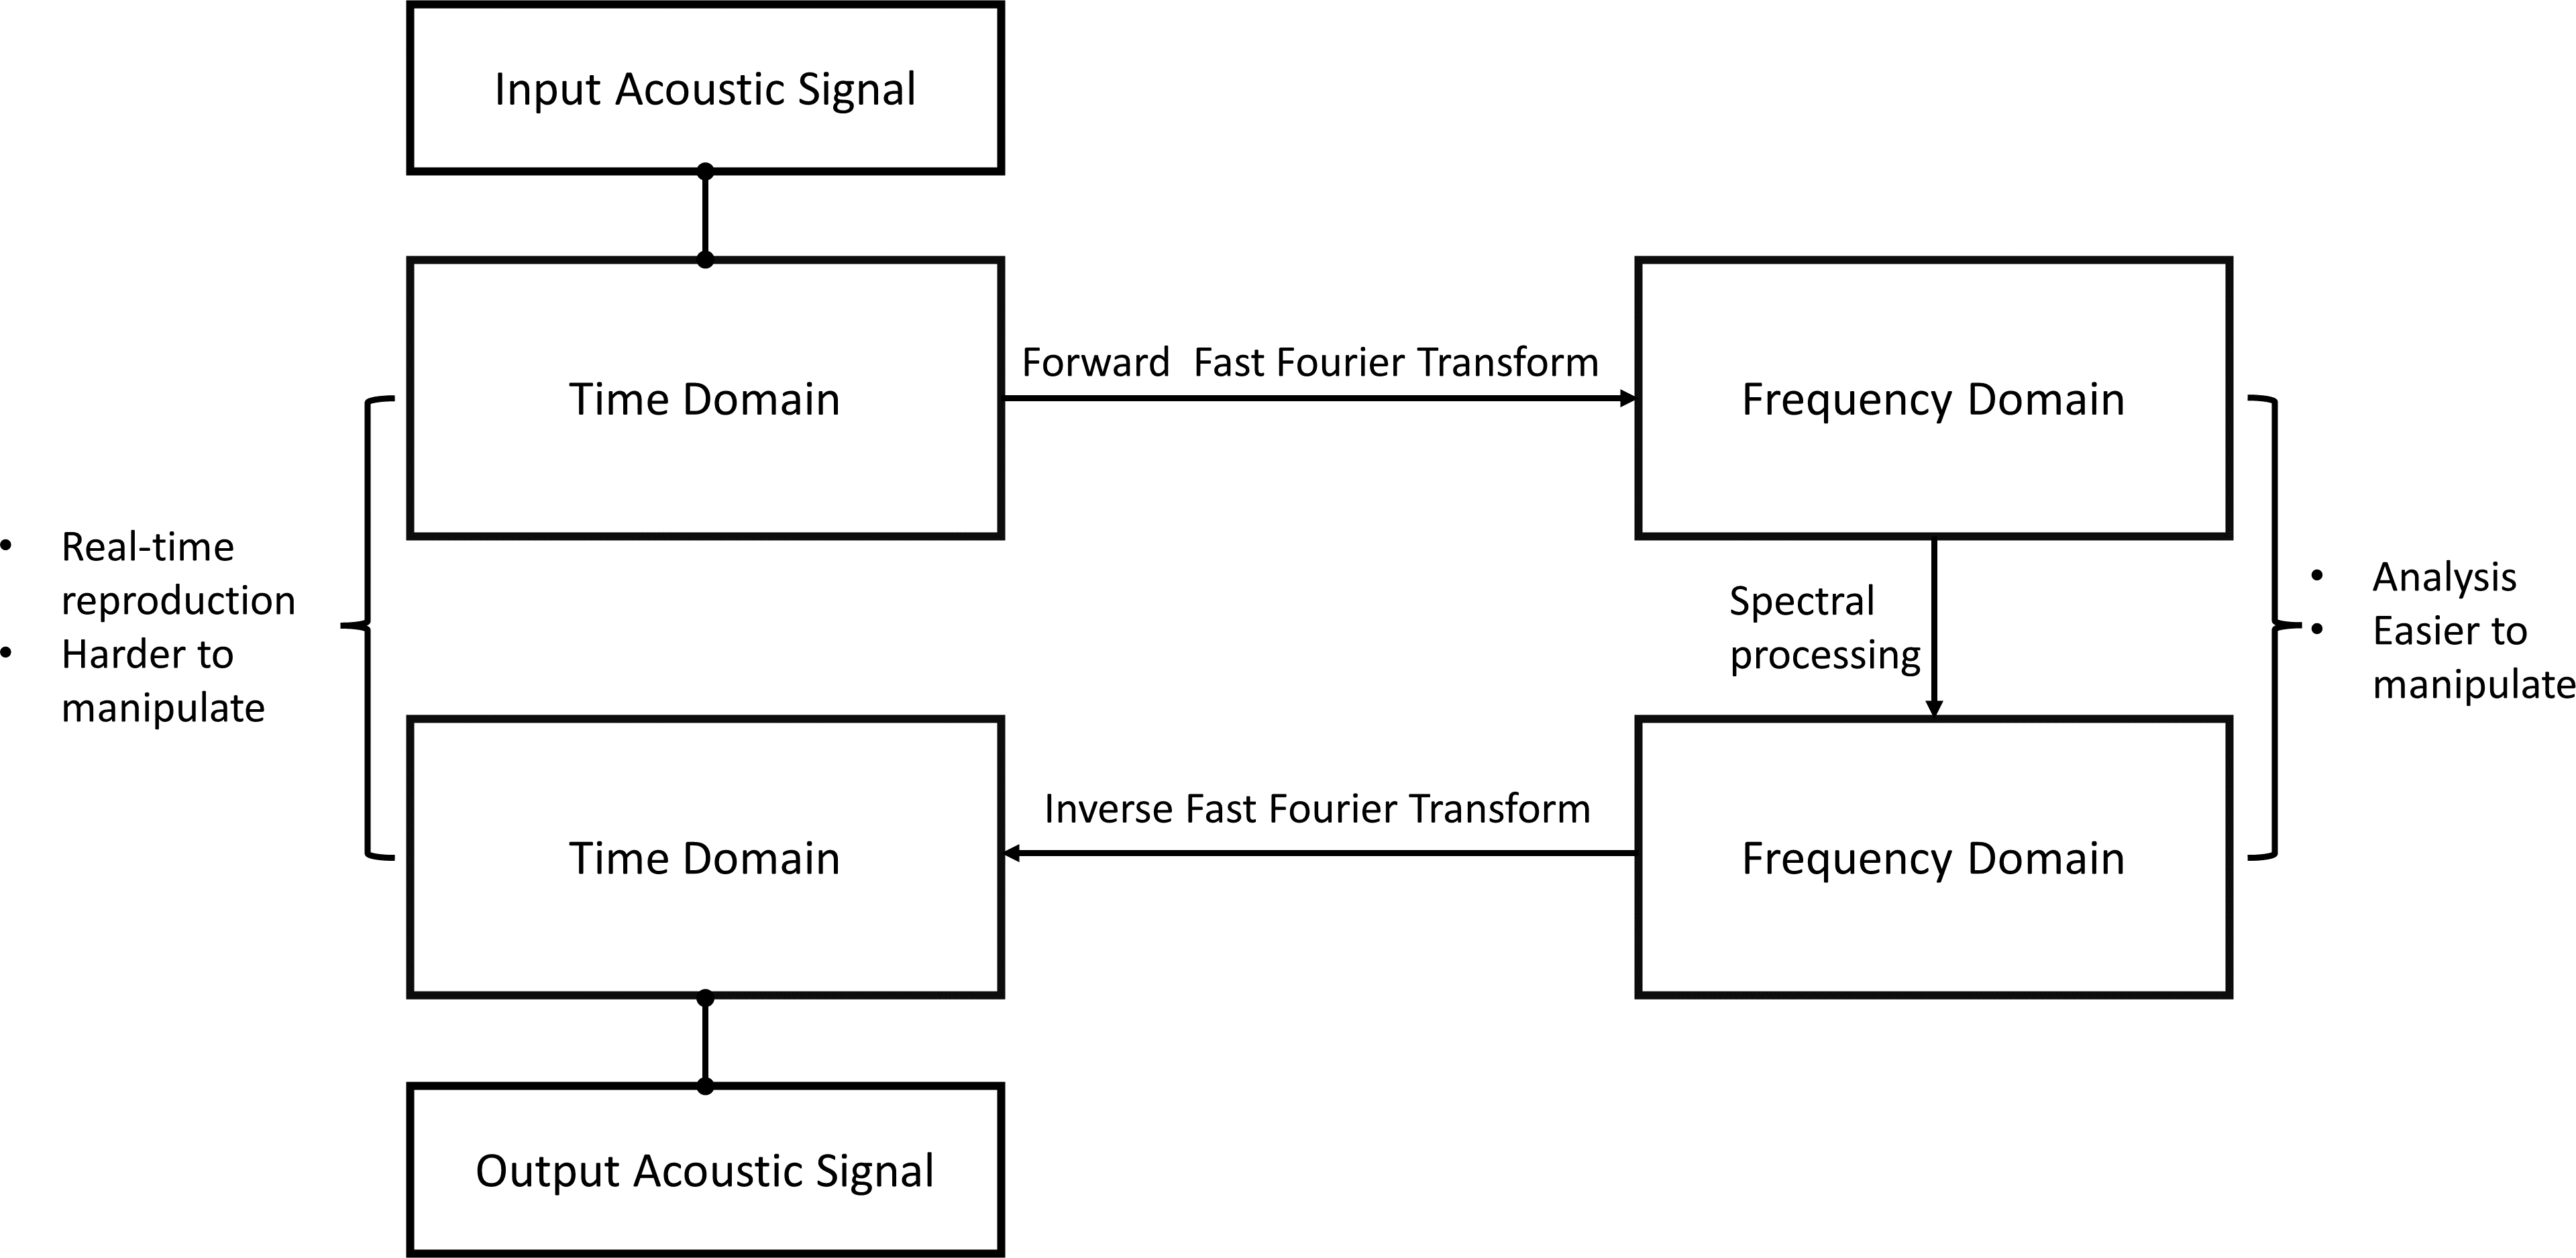
\includegraphics[width=1\textwidth]{DFT}
    \caption{A basic chain for signal processing aimed at analysing or manipulating signal in auralisation, visualisation, or interactive applications. Analysis and processing of digital signals in the time domain is generally a hard task due to the complex nature of the function representing audio. The frequency-domain representation eases analysis and manipulation problems even with the added computational load of transforming between the two domains.}
    \label{fig:DFT}
\end{figure}

\subsection{Image Processing Fundamentals}\label{sec:image-processing}
\begin{itemize}
    \item digital images
    \item basic imge processing techniques
    \item filters
\end{itemize}

\subsubsection{Binaural Room Impulse Responses}\label{sec:ir-definition}
Common approaches to acoustic simulations involve the approximation of acoustic phenomena affecting a sound transmission occurring within a given environment between a sound source and a listener. To represent the result of such a simulation as a measurable process, where the environment is thought of as a dynamic system, Impulse Responses (IR) are used. IRs describe the effect that a system has on a sound transmission as a function of time. From DSP theory, there are several variations of IRs that the fields of immersive acoustics borrow to model several dynamic systems that affect how the human auditory system perceives soundscapes. Figure~\ref{fig:audio_rendering_chain} shows how the auditory display is affected by interconnected systems associated with aspects of the soundscape. Time invariance is the fundamental property of these systems, making it possible to model their effect as an IR by observing their response to a Dirac-Delta function, which is a function whose value is zero except at the origin, where it is infinite. In practical terms, the Diract-Delta function is an infinitely narrow energy spike often used to excite the system and obtain a response across the frequency spectrum over time. In DSP terms, the function is simply represented as a finite sequence of numbers, the Finite Impulse Response (FIR), representing amplitude levels of the output of the system over time, given an input, commonly used to measure the effects of time-invariant linear systems like amplifiers or loudspeakers.\par
In the acoustic domain, the FIR adapts to several tasks, like modelling the acoustic fingerprint of a space with respect to a source and listener by observing, at the listener, a Dirac-Delta-like signal being emitted by the source. Such IR is differentiated from standard IRs and referred to as a Room Impulse Response (RIR); such distinction has emerged from the ongoing research in techniques and methods for measuring responses from real spaces, also due to the chaotic nature of room acoustics and real soundfields \citep{farina07}. 
IRs, as well as measuring the acoustic fingerprint of spaces, can extend as far as measuring the effect of the human auditory system on the perception of the soundscape, and there are methods for modelling how anthropometric characteristics of the human body affect sounds arriving at both ears. Such IRs are defined as Binaural Room Impulse Responses: they extend RIRs by providing individual responses for both ears. BRIRs are a representation of Head-Related Transfer Functions (HRTFs), a function that describes how the anatomic features, rotation, and position with respect to a sound source affect the arrival of sound to the ears. Figure~\ref{fig:rir-spectrum} is an example of a monaural RIR, shown both in the time and frequency domain. 
\begin{figure}
    \centering
    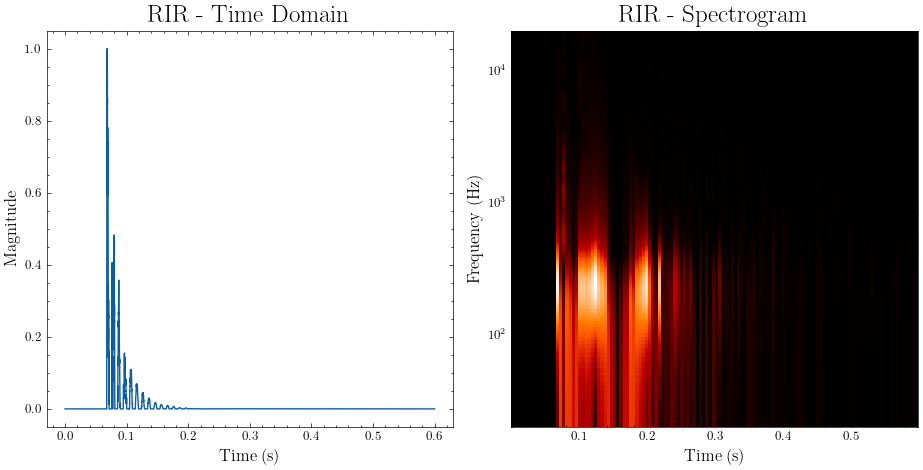
\includegraphics[width=1\linewidth]{rir_spectrum}
    \caption{Both time and frequency-domain, left and right respectively, representations of a Room Impulse Response (RIR). The time domain representation shows the magnitude of sound paths from a sound source to a receiver over time. The frequency domain representation shows how the energy of sound paths is distributed across the frequency spectrum over time, which is visualised with an infrared colour map.}
    \label{fig:rir-spectrum}
\end{figure}

\section{Common Approaches to Immersive Acoustics}
Achieving a convincing immersive acoustic experience is no trivial task, and various techniques and methodologies have been developed to address this complex challenge. These approaches must consider sound's spatial, temporal, and perceptual aspects and the HAS's intricate response to auditory stimuli.

\subsection{3D Sound Reproduction Techniques}
Sound reproduction for immersive acoustics can be defined as a rendering problem concerning providing a listener with synthetic believable auditory stimuli perceived as belonging to a specific space. The rendering is often engineered by adopting a system that has complex scenes and scene elements as input and an acoustic signal as output. 
\begin{figure}
    \centering
    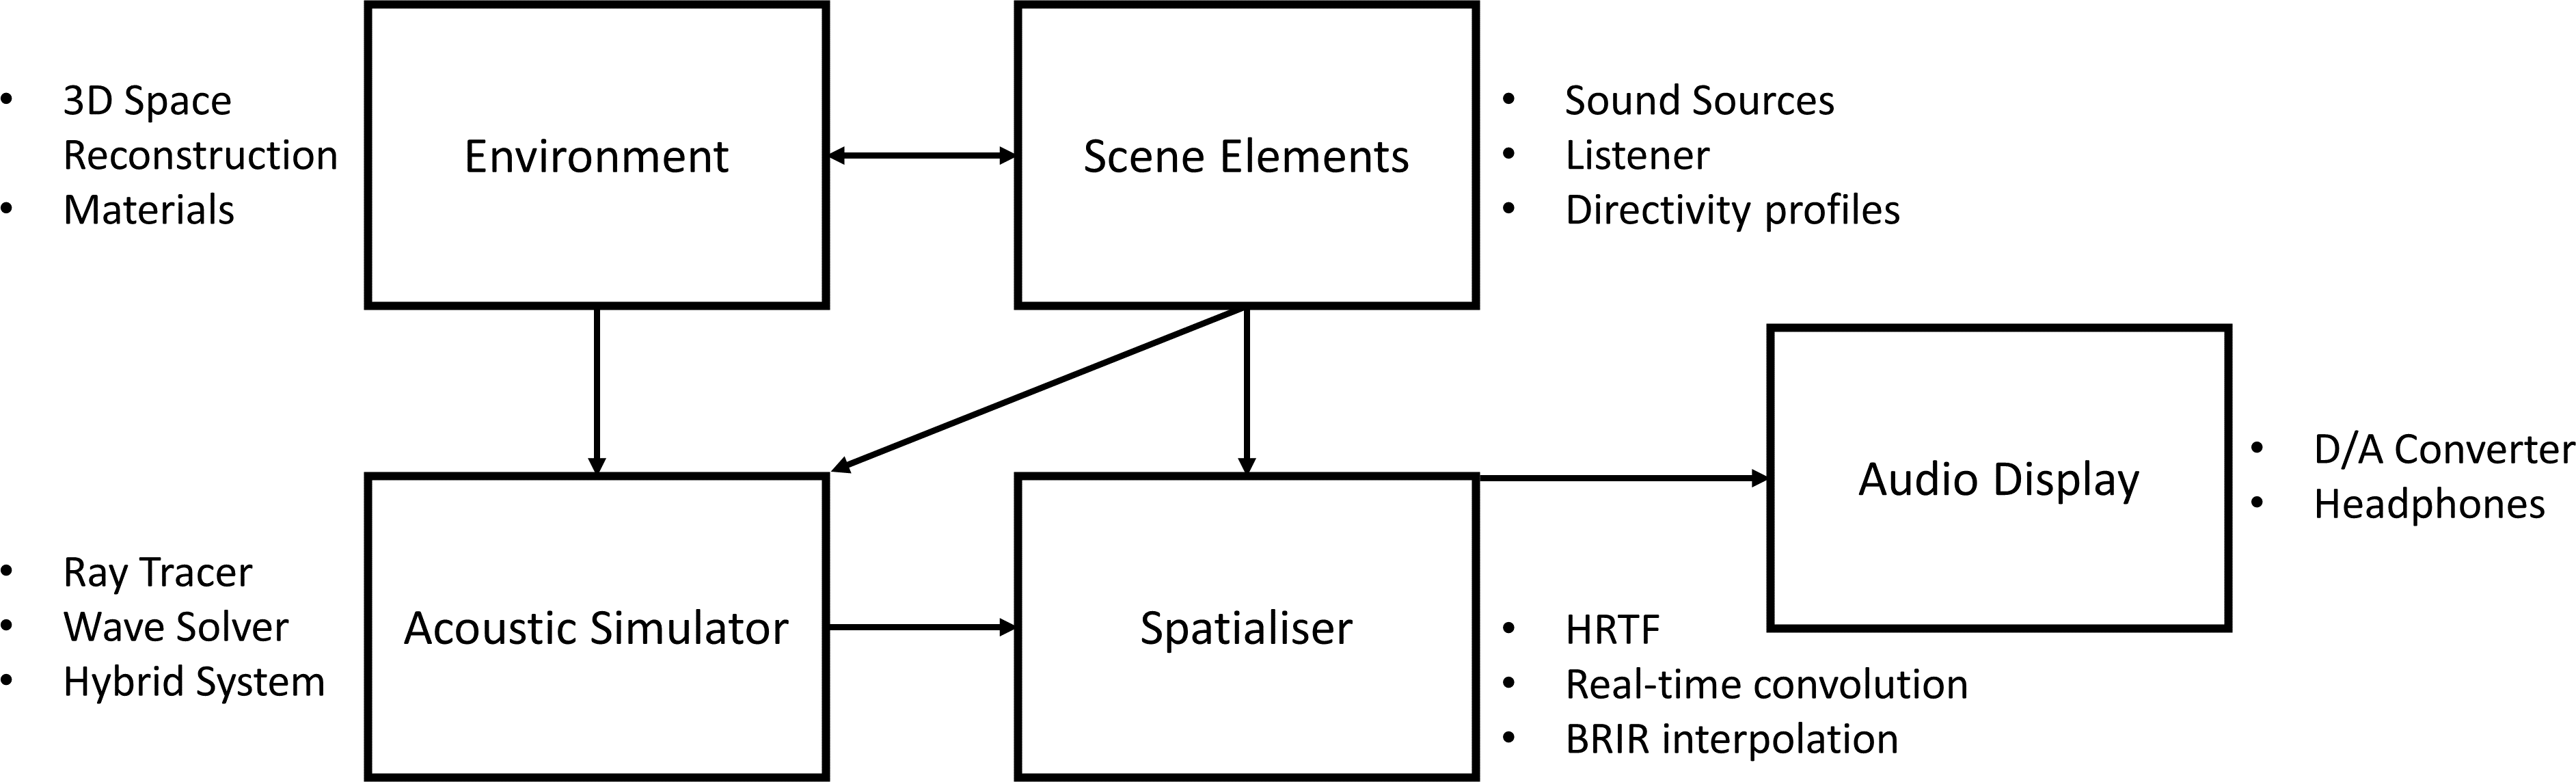
\includegraphics[width=1\textwidth]{spatialiser_system_overview}
    \caption{An example chain of 3D reproduction based on acoustic simulators: an environment is fed into acoustic simulators to produce BRIRs. A spatialiser system consumes these to generate an audio signal considering the listener and scene elements.}
    \label{fig:spatialiser-overview}
\end{figure}

\subsection{Spatial Audio Rendering Algorithms}
\label{sec:real-time-conv}
Audio rendering refers to the process of affecting anechoic audio with acoustic phenomena approximated by simulations. It utilises generated IRs and takes into account the characteristics of a human listener from the perspectives of a sound-perceiving object in a virtual environment and a human receiver with psychoacoustic abilities.

One of the fundamental operations in audio rendering is the manipulation of anechoic audio with a filter encapsulating the acoustic effect of an environment to a sound transmission, expressed as an IR. Given anechoic audio expressed as a digital sequence $x$ containing $x_0, x_1,~\dots,x_n$ elements, and an IR expressed as a digital sequence $h$ containing $h_0, h_1,~\dots,h_n$, through the convolution operation $*$ we can obtain the resulting sequence $y$ containing $y_0, y_1,~\dots, y_n$ samples, expressing the resulting signal with the applied IR. The following mathematical notation shows how a new function is created as a result of the convolution operation:
\begin{equation}
    y[n] = x[n] * h[n].
\label{eq:1d-convolution}
\end{equation}
In audio rendering terms, these functions will often represent an anechoic acoustic signal that is convolved with an IR to apply to create an auralised resulting signal. Given a signal $x$ as a sample sequence of $N$ points and a filter $h$ as a sample sequence of $M$ points, the resulting full convolution $y$ will be a sample sequence of $N + M - 1$ points. Each sample of the resulting $y$ sequence is the sum of the products of both sequences: 
\begin{equation}
    (x * h)[n] = \sum_{m=0}^{M}x[n-m]h[m].
\end{equation}
As shown in Figure~\ref{fig:DFT}, frequency-domain representation makes specific problems easier to solve compared to the time-domain, and convolution is one example because of the summation required in the convolution process. This summation determines the computational complexity of the operation and grows with increasing $M$ filter lengths. One key property of the convolution is that the product of the frequency-domain representation of a signal with the frequency-domain representation of a filter is the frequency-domain of their convolution. Essentially, the added complexity of summation is removed in the frequency domain at the cost of transforming the signals using the DTFT. Hence, audio rendering algorithms use the much faster \acrfull{fft} Convolution, commonly defined as:
\begin{equation}
    (x * h)[n] = IDTFT_N( DTFT_N(x[n]) \cdot DTFT_N(h[n]) ),
    \label{eq:fft_convolution}
\end{equation}
where $DTFT_N$ and $IDTFT_N$ are, respectively, the DTFT and the inverse DTFT of both the signal and the filter calculated over $N$ frequency points.
The Overlap-Add or the Overlap-Save are examples of real-time convolution algorithms often adopted in DSP to implement a wide range of audio effects. They are solutions to the problem of applying BRIR to long signals or to implementing interactive systems, where the listener is displayed rendered audio from a dynamic virtual environment. Thanks to the advances in such algorithms, it is now computationally feasible to manipulate anechoic audio signals with simulated acoustics on the fly, evoking a sense of immersion in the listener due to the auditory stimuli responding to changes in the dynamic environment at interactive rates. \par
The Overlap-Add algorithm adopts the divide-and-conquer approach towards an acoustic signal by segmenting an input digital sequence into multiple parts, processing the individual parts, and assembling the resulting sequence to produce a whole manipulated sequence. The goal is to evaluate Equation~\ref{eq:fft_convolution} over small chunks of audio, storing resulting convolved chunks into a queue from which samples are summed together into an output sequence. \par
Interactive audio rendering algorithms benefit from such systems as they enable on-the-fly convolution with live audio streams, which are generally implemented as a circular audio buffer. In the case of an immersive application, such audio buffers may be storing audio propagating from sound-emitting objects that interact with the user. As illustrated in Figure~\ref{fig:audio_rendering_chain}, spatialiser systems or acoustic simulation systems provide filters in the forms of IRs that can be applied to audio chunks from the audio buffer.
\begin{figure}
    \centering
    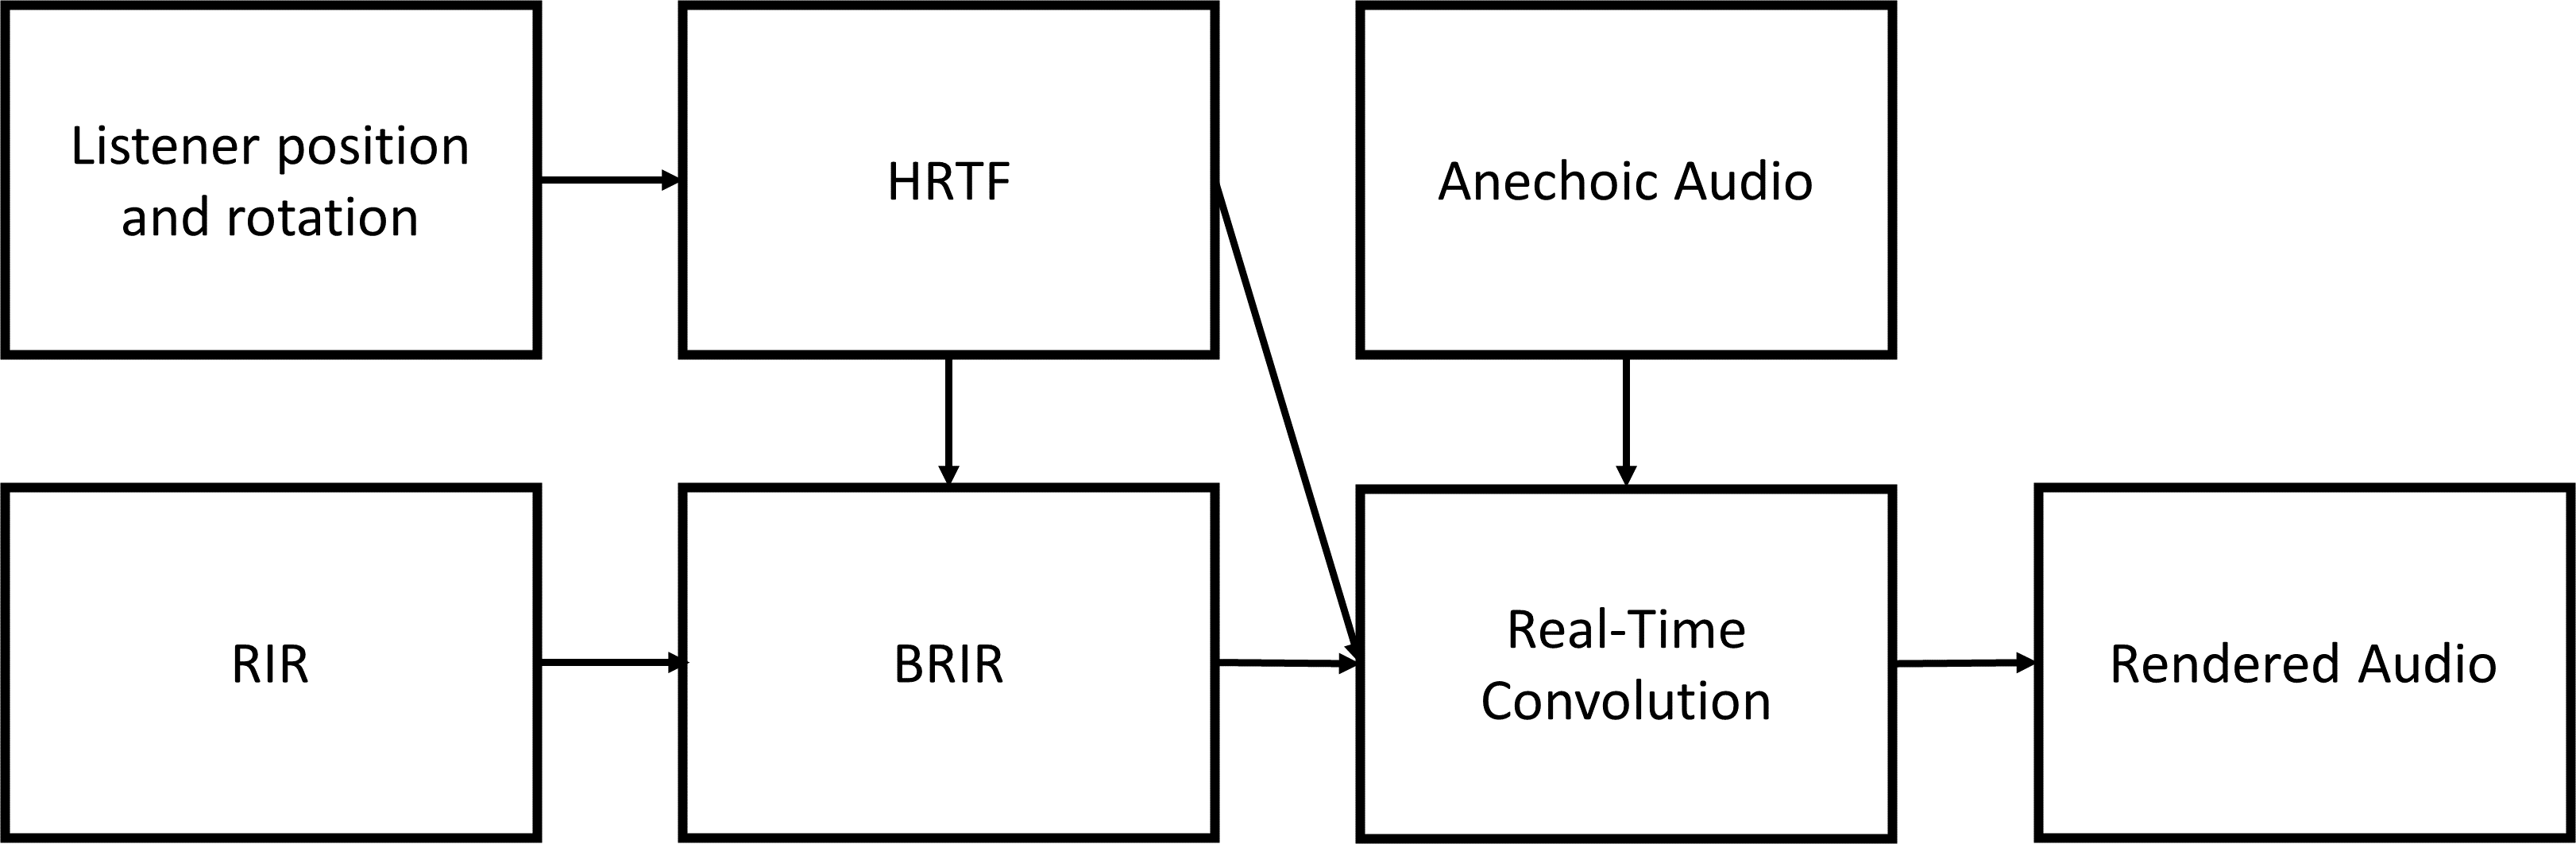
\includegraphics[width=1\textwidth]{audio_rendering}
    \caption{Common spatial audio pipeline: the listener's position and rotation in the scene is used to sample an interpolated HRTF from the currently loaded bank, combined with the generated IR, the real-time convolution algorithm applies the BRIR to an anechoic audio signal. The result is an audio signal arriving at the listener, taking into account their position and rotation with respect to the sound-emitting object in the virtual environment.}
    \label{fig:audio_rendering_chain}
\end{figure}

\section{Auralisations}
The ability to auralising anechoic acoustic signals is one of the fundamental objectives in the domains of acoustics for surveying techniques, acoustics for interactive applications, and acoustics in extended reality. As seen in Section~\ref{sec:DSP-background}, there are DSP techniques that allow the application of acoustic fingerprints onto audio recordings by treating the acoustics phenomena as measurable functions that can be convolved to digital signals, see Equation \ref{eq:1d-convolution}. In higher-level terms, auralisation is the process of experiencing audio stimuli in a simulated soundscape, which can be perceiving an orchestra in a digital representation of a church, approximating how room acoustics affect the sound transmission between the orchestra and the listener in the virtual space. There are factors associated with this process that determine how well the resulting signal is able to fool the listener's auditory system into believing that the auralisation is real. Realism and presence are often a function of the performance of the components in the chain of the 3D audio reproduction system; see Figure~\ref{fig:audio_rendering_chain}.

\subsection{Common methods for Auralisations}
Methods for producing auralisation start from the creation of an environment, which is the first component of the system in Figure~\ref{fig:audio_rendering_chain} hosting the virtual sound-emitting objects, e.g. an orchestra, and the virtual sound-receiving objects, e.g. the listener. In computers, environments are generally represented using a broad range of computer graphics techniques, from simplistic Computer-Aided Design (CAD) to fully-featured virtual worlds engineered in modern game engines. Such a statement blurs the definition of a virtual environment, as one could represent a room by creating a photorealistic 3D model or by simply drawing a cuboid. Research on acoustic simulations conducted over the last decades has expanded towards defining what is required from a virtual environment to produce a believable simulation. The representation of the environment geometry is a determinant of the resolution and perceptual quality of the acoustics simulation results, and, as a general rule, the higher the level of details expressed by the geometry, the more accurate the acoustic simulator is able to simulate how sound interacts with the environment. However, beyond certain levels of details, the increase in resolution does not have a significant perceptual response \cite{pelzer2010frequency}.\par
Combined with advances in real-space scanning technology and user-friendly 3D reconstruction software, it is now possible to create appropriate virtual environments for acoustic simulations without requiring expert computer graphics engineering knowledge.\par

\subsubsection{Geometrical Acoustics Modelling Techniques}\label{sec:bg-raytracing}
Geometrical acoustics is a family of acoustic modelling methods based on representing propagating sound waves with geometrical primitives, such as rays or cones. The foundations of these methods have sound propagating as straight lines, as opposed to moving particles, approximating the complex nature of acoustic energy transfer but neglecting phenomena related to the wave phenomena.

\citep{savioja2015overview}.

Ray-based techniques, wave-ray hybrid techniques, and wave-based techniques have emerged as prominent methods to generate impulse responses in the field of acoustics, each contributing to understanding how sound propagates within a given space. Ray-based techniques, rooted in geometric acoustics, simulate sound by tracing rays that emanate from a source and bounce off various surfaces within a space. This method creates echoes and reverberations, contributing to the overall impulse response. Notably, it offers efficiency as it is computationally less demanding than wave-based techniques, making it suitable for real-time applications or large-scale spaces often found in cultural heritage contexts. The geometrical nature of ray-based methods allows for easier integration with virtual reconstructions of space and dynamic geometry, and the method's inherent flexibility makes it easily adjustable to different acoustic scenarios. \cite{vorlander2008simulation}

\subsubsection{Hybrid Modelling Techniques}
On the other hand, wave-ray hybrid techniques present a more complex picture, combining aspects of ray-based and wave-based methods. Rays are utilised to model the high-frequency components of the sound, while wave equations handle the low-frequency behaviour, attempting to capture the best attributes of both methods. However, the hybrid nature often means more computational resources are needed, and it might not always be the most suitable choice for fast applications where platforms offer limited computational resources. \cite{hulusic2012acoustic}

\subsubsection{Wave-based Modelling Techniques}
Wave-based techniques stand out for their precision, solving the wave equation to simulate how sound waves propagate through space, accurately modelling diffraction, scattering, and other complex wave phenomena. While highly accurate, wave-based techniques often require substantial computational resources, making them less suited for real-time or large-scale applications. \cite{hamilton2017fdtd, raghuvanshi2014parametric}.\par

\subsubsection{Summary}
Ray-based techniques offer a compelling option for interactive applications. Their computational efficiency, relative simplicity, and adaptability in handling various scenarios effectively capture the essential acoustic characteristics of sounscapes. Unlike wave-based or hybrid methods, ray-based techniques can easily adapt to dynamic environments, aligning with the objectives of this work and constraints often found in \acrshort{ar} platforms. Therefore, while the high accuracy of wave-based methods or the comprehensive nature of hybrid methods may have specific applications in areas of high-fidelity and complex propagation effects, it is the ray-based techniques (such as those employed by acoustic simulation software such as ODEON) that generally stand out as the most appropriate choice for fast and efficient acoustic simulation in immersive applications.

% ---------------------------------------------------------------------------------
% * Virtual Environments
% ---------------------------------------------------------------------------------
\section{Virtual Environments}
Room acoustics simulations may involve the concept of virtual environments to represent sound-emitting objects, receivers, and space where these exist. Computer games technology has shaped the definition of virtual environments over decades of development and progress.

\subsection{Representation of Virtual Environments}
Graphics rendering pipelines display objects of a complex scene to viewers, determining the appearance of materials and geometry of the environment. In VEs, meshes are composed of triangles enabling game engines to organise geometry based on the semantics of scene objects. For E.g. a mug can be represented by triangles grouped in a mesh. They are essentially a network of triangles that connect, having adjacent vertices, to form objects. They are responsible for transforming the scene geometry and applying further processing, such as rasterisation, which generates fragments from geometry combined to create frames. A series of frames generated at interactive rates compose a frame buffer that allows users to experience scenes in real-time. Graphics pipelines describe geometry as vertices and triangles, applying shading techniques to control the appearance of surfaces depending on their lighting conditions and the viewer’s spatial position. Here, texture images can also define the appearance of objects' geometry by painting their surfaces and controlling transparency \citep{mcallister2002efficient, marschner2015fundamentals}.\par
Textures can determine the appearance of material composing objects in a scene adopting two-dimensional images. Texture mapping uses colour and transparency information contained in these images to paint triangles forming the geometry. Texture coordinates provide graphics pipelines with enough information to paint meshes.

\subsection{Handling of Complex Scene Geometry}\label{sec:bg-geometry-handling}
Implementing multimodal interactions in \ACRshortpl{ve} often requires handling and performing operations on the scene geometry, including searching interactions between entities and the environment. In computer games, physics systems are often fundamental components enabling game mechanics and interactions, which often involve computing intersections between scene entities and the environment. With the growing density of environment geometry and complexity of the scene elements, the computational requirements associated with evaluating these geometry searches have grown, demanding optimal solutions across the space and time domains.\par
The goal of geometry handling systems is to allow searching intersections between volumes or primitives, such as rays or frustums, and the scene geometry and the engineering design of such systems are closely related to data structures and algorithm design. Data structures space and time complexity
\begin{figure}
    \centering
    \begin{subfigure}[t]{0.3\textwidth}
       \centering
       
\includegraphics[width=\textwidth]{bvh1}
       \caption{Triangulated Mesh}\label{fig:sub_bvh1}
    \end{subfigure}
    \hfill
    \begin{subfigure}[t]{0.3\textwidth}
       \centering
       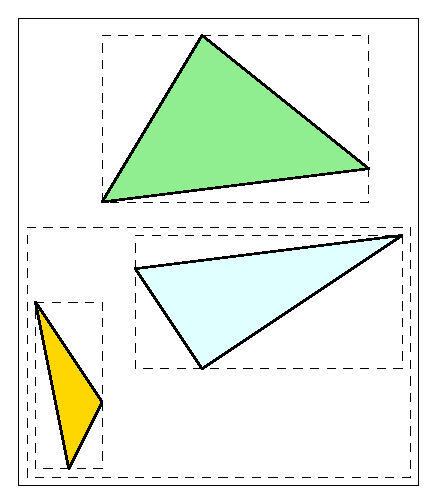
\includegraphics[width=\textwidth]{bvh2}
       \caption{Bounding Volumes}\label{fig:sub_bvh2}
    \end{subfigure}

    \begin{subfigure}[t]{0.8\textwidth}
        \centering
        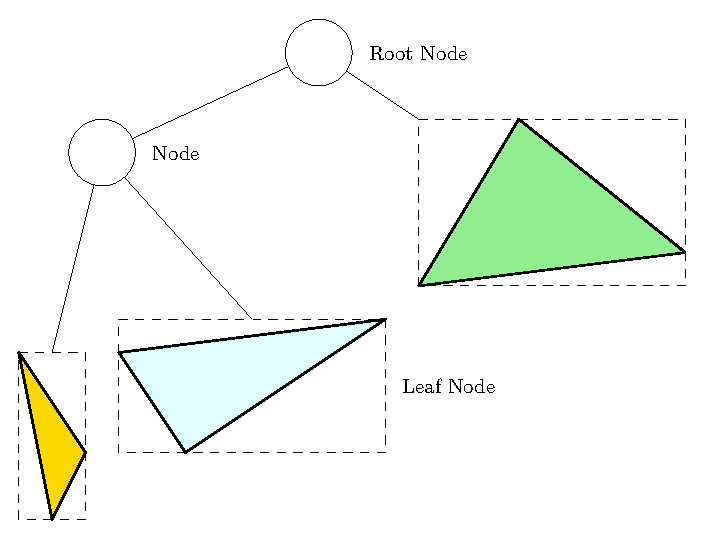
\includegraphics[width=\textwidth]{bvh3}
        \caption{Tree}\label{fig:sub_bvh3}
    \end{subfigure}
    \caption{A bounding volume hierarchy constructed on a given input scene represented as a triangulated mesh (a). Bounding volumes encapsulate mesh primitives, (b), which then represent nodes of the tree, (c).}\label{fig:bvh-diagram}
\end{figure}


\subsubsection{Binary Space Partitioning}
One of the first approaches in handling and indexing scene geometry in \acrshortpl{ve} is \acrfull{bsp}, which, motivated by performance aspects and limited computational resources available during the early developments of rendering pipelines in the field of computer graphics \citep{fuchs_bsp}. \acrshortpl{bsp} allow graphics pipelines to organise the order of scene elements before drawing them or to determine the visibility of surfaces.\par
The goal of \acrshortpl{bsp} is to index and search scene elements or geometry primitives, part of a given input scene. The technique works by subdividing the Euclidean space in which scene elements exist. The space is divided by partitioning planes, separating scene elements based on which side of the plane they exist. The process repeats recursively, subdividing space with further partitioning planes. Several criteria can determine the number of further subdivisions, such as the minimum size of regions generated by space subdivisions or the indexing complexity and granularity required for indexing and searching operations.\par
With subdivided regions obtained with partitioning planes, a binary tree, similar to the diagram shown in Figure~\ref{fig:bvh-diagram}, where a root node refers to the entire scene and branches into the first space subdivision, which recursively branches into further subdivisions, until a ``leaf'' region. A leaf region can hold a scene element, a geometry primitive, or a subset of primitives from the set of primitives representing the input scene.\par

\subsubsection{Bounding Volume Hierarchies}
A \acrfull{bvh} is a method closely related to \acrshort{bsp} for handling scene geometry that optimises intersections between rays and the scene by adopting a binary tree to subdivide primitives that compose the scene geometry. A \acrshort{bvh} can represent a scene by constructing a binary tree partitioning geometry primitives into a hierarchy of disjoint sets. In physically-based rendering applications, mesh triangles are often the primitives indexed by the constructed tree; see Figure~\ref{fig:bvh-diagram} \citep{pharr2023physically}.\par
In a tree, bounding volumes are generated to fit primitives from a given triangulated mesh (Figure~\ref{fig:sub_bvh1}) and aggregated based on proximity (Figure~\ref{fig:sub_bvh2}). Bounding volumes encapsulating multiple primitives generate branches, and recursively, branches are encapsulated in volume until a root volume fits the entire input scene. A constructed tree (Figure~\ref{fig:sub_bvh3}) can be queried and traversed by navigating branches from the root node to primitives within leaf nodes.\par
Thanks to branch subdivisions, ray-volume intersection tests performed on nodes allow filtering out entire segments of the scene, reducing the set of primitives that potentially intersect the ray to a subset of the input scene triangle set and improving the space complexity of the operation, much like in \acrshort{bsp} techniques. Recent research trends are exploring tree rotations and balancing of branches in real-time, optimising search operations even further, and allowing the tree to reflect dynamic changes to the scene geometry \citep{kopta2012fast}.
 
\subsection{Sound Sources in Virtual Environments}
Representing space in virtual environments, capturing real space and synthetic scenes.
- Game Engine architecture book                             

\subsection{Materials}
\begin{figure}
    \centering
    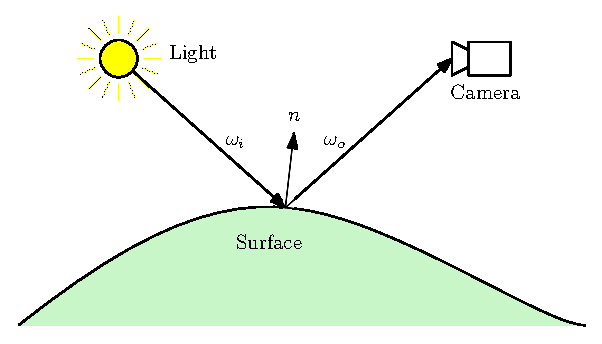
\includegraphics[width=1\textwidth]{brdf1}
    \caption{A simplistic material system visualised as a ray of light emitted by a source and colliding with a surface. The ray reflects around a surface normal and is detected by a virtual camera.}\label{fig:material-vis}
\end{figure}
In computer graphics and multi-modal rendering, assigning physical properties to surfaces of the scene geometry has been addressed with the definition of materials. The definition of materials is often intrinsic to the rendering technique and to the engineering design of the rendering apparatus. In physically-based graphics rendering techniques,~\cite{pharr2023physically} define materials as a
\begin{quotation}
    ``description of its appearance properties at each point on the surface''.
\end{quotation}
\subsubsection{Materials in Rendering Pipelines}
Rendering pipelines often model how surfaces in complex scenes reflect and respond to propagating energy by employing \acrfullpl{brdf}. In the light domain, rendering techniques often model reflected energy as a function $f_r(p, \omega_i, \omega_o)$ of a $p$ \acrshort{brdf}, an incoming direction $\omega_i$ and an outgoing direction $\omega_o$. A simplified diagram in Figure~\ref{fig:material-vis} shows how energy transmits from a light source and is sampled by a virtual camera, with a surface reflecting the light ray around the surface normal at the collision point. Though, materials in the real world have unique physical properties affecting reflectance, absorptions, or diffusion of incidental light, deviating from the idealised model shown in the Figure.\par
A material using a reflectance function can model realistic behaviour, allowing surfaces to express varying physical attributes like roughness or metallic characteristics. Figure~\ref{fig:brdf-vis} shows example functions simulating a rough and a glossy material, Figure~\ref{fig:brdf1}~and~\ref{fig:brdf2} respectively. These examples show \acrshortpl{brdf} modelling the scattering of energy caused by the rough surface and the glossy reflections caused by a mirror-like surface.\par
\subsubsection{Materials in Sound Rendering}
Defining materials translates to the acoustics domain, applying closely related principles defined in the visual domain. \ACRshort{ga} methods often share the same approach shown in Figure~\ref{fig:material-vis} by considering sound in \acrshortpl{ve} as propagating rays (or other geometry primitives) colliding with surfaces that reflect energy based on attributes assigned to the surface.\par
In real soundfields, acousticians and architects often plan the presence of certain materials to control aspects of sound propagation within a given environment. Studies show that strategic placements of surfaces with high acoustic absorption characteristics can have a positive subjective influence on perception in environments, improving the clarity of acoustic information transmitted within the space \citep{arvidsson2021subjective}. Absorption panels, diffusers, or bass traps are some example materials and surfaces that acousticians use to control how acoustic energy reflects around the environment, controlling parameters like $T_{30}$ or $T_{60}$ reverberation metrics or $C_{50}$ and $D_{50}$ clarity and definition metrics, respectively.\par
Modern game engines and acoustic simulation software aim to replicate the behaviour of these surfaces by encoding acoustic characteristics to scene geometry representing an environment. In \acrshort{ga} simulation methods, material characteristics like absorption or scattering coefficients can influence of geometry primitive simulating propagating sound and interact with the environment, similarly to \acrshortpl{brdf} \citep{rindel2000use}. Finally, acoustic material can encode frequency-dependent acoustic information, often expressed around \acrfull{erb} frequency region, to consider aspects of the \acrshort{has}. Chapters~\ref{ch:Materials}~and~\ref{ch:acousticrendering} will discuss the use of materials in the context of the overarching aim of this thesis.

\begin{figure}
  \centering
    \begin{subfigure}[t]{0.49\textwidth}
       \centering
       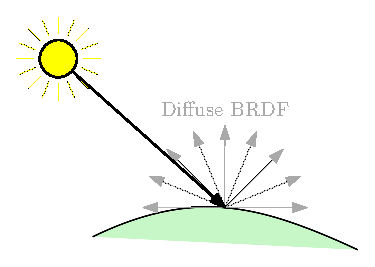
\includegraphics[width=\textwidth]{brdf2}
       \caption{Rough Material}\label{fig:brdf1}
    \end{subfigure}
  \hfill
    \begin{subfigure}[t]{0.49\textwidth}
       \centering
       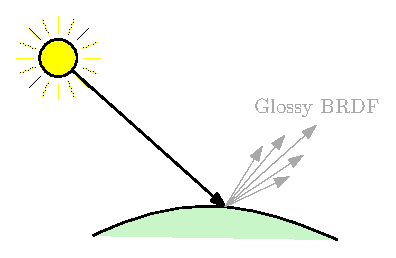
\includegraphics[width=\textwidth]{brdf3}
       \caption{Glossy Material}\label{fig:brdf2}
    \end{subfigure}
  \caption{Example \acrshortpl{brdf} applied to a surface, defining a rough material (a) and glossy material (b). These functions emulate how properties of real surfaces respond to colliding light: glossy materials will reflect energy specularly, whereas uneven rough surfaces will cause diffuse scattering.}\label{fig:brdf-vis}
\end{figure}

% Absorption, diffusion, scattering, and physical properties of materials.

\section{Deep Learning}
Subsequent chapters of this thesis will leverage deep learning techniques to solve a subset of problems associated with developing a system targeting the overarching aim. Specifically, acoustic materials are central to applying the system to realistic, complex scenes, as they contribute towards the perceived quality and realism evoked by the auditory display. The problem arises from the complexity of mapping the appearance of surfaces within the complex scene to acoustic materials. Many factors in complex virtual environments influence the appearance of surfaces, making it hard to distinguish surfaces and map them against acoustic materials automatically.\par
Deep learning is a subset of machine learning comprising techniques and pipelines to address such mapping problems by learning from examples and providing a generalised model for unseen cases. The potential of deep learning lies in the feature extraction process, allowing models to learn from examples influenced by many factors. The term deep learning is associated with the feature extraction process, delegated to layered feature extraction components composing the model.\par
The goal of a model is to provide inference on unseen data based on training on a set of representative examples, emulating basic human abilities that are hard to programmatically engineer in computers.

\begin{figure}
    \centering
    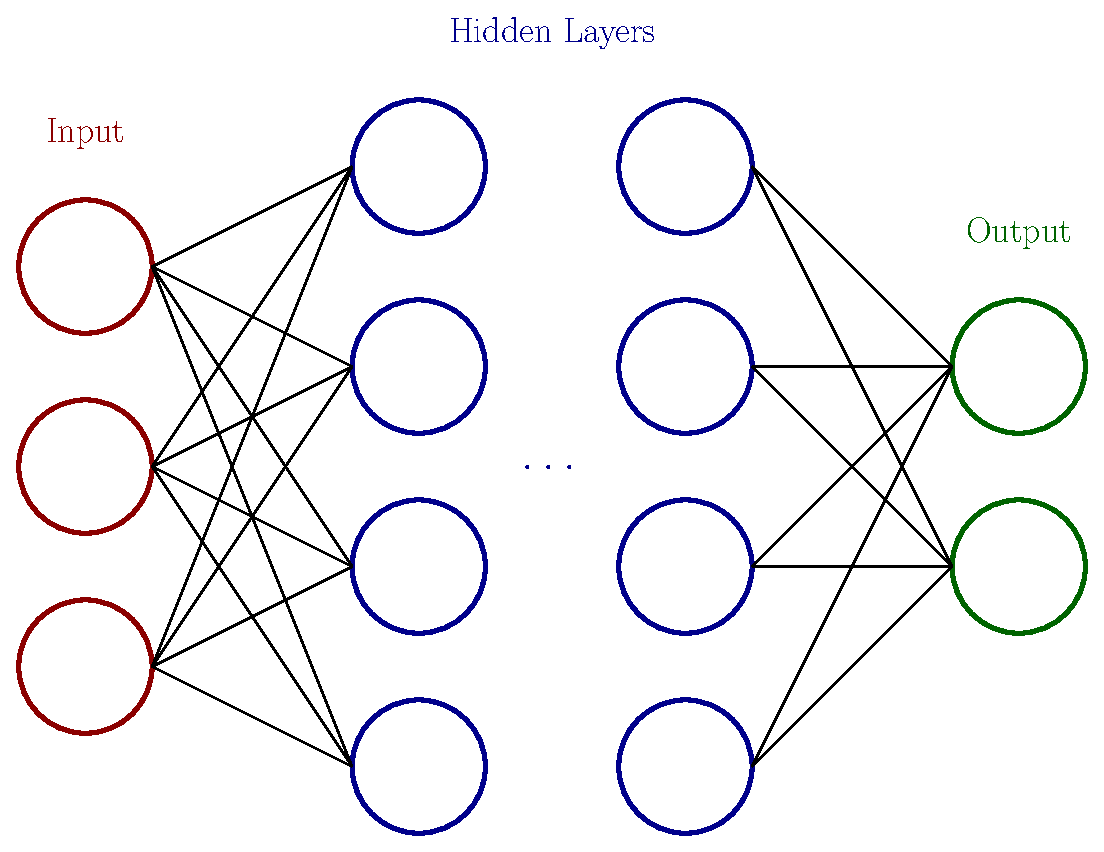
\includegraphics[width=1\textwidth]{nn}
    \caption{A visualisation of a basic neural network with fully-connected hidden layers.}\label{fig:nn}
\end{figure}

\cite{goodfellow2016deep}
General Machine Learning Tasks

\begin{itemize}
    \item classification
    \item regression
    \item synthesis and sampling
    \item extrapolation
\end{itemize}

TPUs and specialised hardware for neural nets.

\subsection{Applications Within Immersive Media}
Deep learning techniques are becoming increasingly popular in virtual environment pipelines due to the flexibility and potential to adapt to various tasks. 

\subsection{Object Detection and Segmentation}
Detecting the presence of certain objects in an image represents a milestone in the development of \acrshortpl{cnn} and computer vision techniques as it emulates a basic task of the human visual system. Due to the nature of image representations in computers, as described in Section~\ref{sec:image-processing}, recognising entities depicted by images is a central problem in computer vision \citep{szeliski2022computer}. Classic computer vision algorithms have approached the problem by providing algorithms to recognise patterns programmatically by filtering the image or scanning for certain features. Thanks to advances in \acrshortpl{cnn}, object detection was addressed by extracting features using deep layers and learning from annotated examples expressing a set of classes captured in various contexts.\par
Pioneering large-scale labelled datasets, such as the work by~\cite{deng2009imagenet} on ImageNet, enabled object detection networks to improve their efficiency and abilities of recognising classes. Of pioneering importance is~\cite{Redmon_2016_CVPR}'s You Only Look Once (YOLO) network that introduced a state-of-the-art solution able to recognise thousands of classes with high accuracy and precision.

Similarly to object detection, the problem of image segmentation \cite{minae_segmentation} (review of techniques)


\begin{itemize}
    \item 3D scene segmentation and recognition \cite{kalogerakis20173d}
    \item pose estimation \cite{andriluka20142d}
    \item scene reconstruction \cite{patow2003survey}
    \item sound source separation \cite{virtanen2006sound}
    \item audio scene understanding \cite{abesser2020review}
    \item sound propagation \cite{liu2022sound}
    \item perceptual similarity \cite{Dolhasz_2020_CVPR}
    \item agency in games \cite{yannakakis2018artificial}
\end{itemize}

\subsection{Audio Scene Understanding and Source Separation}
Reasoning and performing tasks on auditory information are analogous to computer vision problems due to the same nature of digital representations.

Sound source separation, also known as audio source separation or audio source separation, is a process in audio signal processing that aims to separate individual sound sources from a mixture of sounds. It is the task of isolating and extracting specific audio sources from a recording where multiple sound sources are present. In many real-world scenarios, such as music recordings, conversations, or environmental recordings, multiple sound sources contribute to the overall audio signal. Sound source separation techniques are employed to enhance the clarity and quality of individual sources, making it easier to analyze, process, or manipulate specific elements within the audio.

\section{Conclusions}

The current state of interactive sound rendering allows for fast acoustic simulations, even on platforms with limited computational budgets, approximating the soundfield of any given environment, where a listener can experience realistic auditory interactions with virtual sound sources \citep{lakka2018spatial, hulusic2012acoustic}. Sound rendering can be considered a fundamental component of computer games technology, responsible for reproducing everyday sound emitted by objects or agents in a virtual scene and perceived by a listener. This poses the challenging task of reflecting basic acoustic principles to render such auditory interactions realistic. In the real world, sound propagates from a sound source to a listener and interacts with objects in the environment and with the environment itself arriving at the listener's ears \citep{kuttruff2016room}. Sound cues alone are sufficient to enable users in Virtual Environments (VEs) to pinpoint locations of sound-emitting entities in a scene by using auditory sound localisation, a natural ability associated with the human auditory system \citep{lokki2005navigation, rubio2017immersive}. \par
As the acoustic principles that govern how sound propagates in space are difficult to reproduce in digital systems, many methods exist, providing variable orders of approximations, depending on the application. Such approaches emulate the wavefield of an environment, simulating how sound interacts with boundaries and scene objects. A subset of these can reproduce phenomena of sound, such as diffraction, reflection, and refraction, which are determinants of realism as they emulate how waves bend around obstacles. Such phenomena make the simulated wavefield dependent on the accuracy of scene geometry and materials represented in a VE. \par
There is a large tree of techniques and methods to simulate sound propagation, reflecting acoustic properties to any given sound source in a VE, adapting to perceptual requirements and computational budgets available \cite{doukakis2019audio}. As a general rule, the more computational budget available, the more complex techniques can be employed, allowing realistic sound rendering. Finite-difference Time Domain (FDTD) approaches shown by \cite{hamilton2017fdtd}, or wave-based by~\cite{raghuvanshi2014parametric} methods, on this end of the spectrum, obtain high degrees of accuracy and realism, but often require pre-computation stages or GPU implementations to produce acoustic simulations at interactive rates. On the other end of the spectrum, there are fast geometrical acoustics methods, widely adopted in real-time applications due to their low computational requirements and highly parallelisable implementations \citep{cowan2010gpu}, which reduce simulated sound waves to rays or beams, that are much simpler to compute. Finally, hybrid methods also exist to combine the strengths of the main families. \par
Acousticians and engineers have always employed classic sound rendering to solve practical problems as it requires the work of experts to adjust parameters and define the acoustic characteristics of a virtual scene. A constant here is the requirement of an accurate description of the environment, detailing the geometry of architectural components and objects contained within with acoustic information such as acoustic energy absorption, reflection, or scattering --- this is essential to model the behaviour of sound waves interacting with the environment. \par
Only recently, with the increase of processing power available in computers, it has gained popularity in computer games and immersive technology for entertainment and serious applications \citep{zhang18}. Augmented Reality (AR) technology can particularly benefit from this as the increase in processing allows sound rendering on mobile devices, enabling listeners to experience virtual sound sources propagating in the reconstruction of real geometry, which is the main avenue that the planned thesis work aims to explore. \par

% Acoustic materials
% Deep learning for acoustic materials
% Next up: lit review




